\documentclass{beamer}

\mode<presentation> {
\usetheme{bits}
%\setbeamertemplate{Fluid Mechanics} % To remove the footer line in all slides uncomment this line
%\setbeamertemplate{footline}[page number] % To replace the footer line in all slides with a simple slide count uncomment this line
%\setbeamertemplate{navigation symbols}{} % To remove the navigation symbols from the bottom of all slides uncomment this line
}
\usepackage{graphicx} % Allows including images
\usepackage{booktabs} % Allows the use of \toprule, \midrule and \bottomrule in tables
\usepackage[english]{babel}
\usepackage{listings,multimedia}
\usepackage{multimedia}
\usepackage{ulem}
\usepackage{chemfig}
\usepackage{amsmath}
\usepackage{mathtools}
\usepackage{commath}
\usepackage{float}
\usepackage{caption}
\usepackage{multirow}
\usepackage{amssymb}
\usepackage[FIGTOPCAP,hang,nooneline]{subfigure}
\usepackage{tikz}
\usepackage[labelformat=empty]{caption}
\renewcommand{\thesubfigure}{}
\newcommand{\lmath}[1]{$\mathrm{#1}$}
\newcommand{\lbmath}[1]{$\mathbf{#1}$}

\newenvironment{descrsf}[1]
  {\begin{list}{}{\renewcommand{\makelabel}[1]{\textsf{##1}\hfil}
                  \setlength{\itemsep}{0.5em}
                  \setlength{\parsep}{0pt}
                  \settowidth{\labelwidth}{\textsf{#1}}
                  \setlength{\labelsep}{10pt}
                  \setlength{\leftmargin}{\labelwidth}
                  \addtolength{\leftmargin}{\labelsep}
                  \providecommand{\descriptionlabel}[1]%
                  {\hspace{\labelsep}\textsf{#1}}
                 }
  }
  {\end{list}}
  \newcommand\blfootnote[1]{%
  \begingroup
  \renewcommand\thefootnote{}\footnote{#1}%
  \addtocounter{footnote}{-1}%
  \endgroup
}

\newcommand{\addlogo}{\hfill
\includegraphics[width=.2\textwidth,height=0.05\paperheight,trim=0 -0.65cm 1.5cm 2cm]{brand_strip_logo.png}}
\newcommand{\bitstitle}[1]{\makebox[\framewidth]{#1 \addlogo}}

%----------------------------------------------------------------------------------------
%	TITLE PAGE
%----------------------------------------------------------------------------------------

\title[Incompressible flow]{Incompressible flow in pipes and channels} % The short title appears at the bottom of every slide, the full title is only on the title page
\author{Eldhose Iype} % Your name
\institute[BITS Pilani, Pilani Campus]{} % Your institution as it will appear on the bottom of every slide, may be 
\date{\today} % Date, can be changed to a custom date

\begin{document}
\begin{frame}
\titlepage
\end{frame}


\setbeamercovered{transparent=0}
\begin{frame}
\frametitle{\bitstitle{Shear-stress distribution}}
\begin{center}
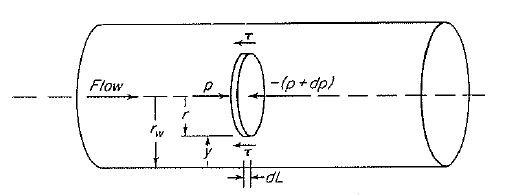
\includegraphics[scale=0.3]{figures/flow_pipe.png}
\end{center}\pause
Applying momentum balance for the disc shaped fluid element
\begin{align*}
\frac{dp}{dL}+\frac{2\tau}{r} = 0
\end{align*}\pause
In steady flow, either laminar or turbulent, the pressure at any given cross section of a stream tube is constant, so that $dp/dL$ is independent of $r$. \pause
At the wall, the above equation becomes
\begin{align}
\frac{dp}{dL}+\frac{2\tau_w}{r_w} = 0
\end{align}\pause
\end{frame}
\setbeamercovered{invisible}

\setbeamercovered{transparent=0}
\begin{frame}
\frametitle{\bitstitle{Shear-stress distribution}}
Combining both equations, we get
\begin{align*}
\frac{\tau}{r}  = \frac{\tau_w}{r_w} 
\end{align*}\pause
\begin{center}
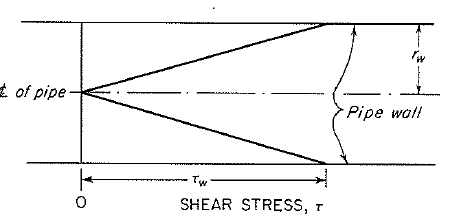
\includegraphics[scale=0.5]{figures/shear_stress_pipe.png}
\end{center}
\end{frame}
\setbeamercovered{invisible}

\end{document} 